 
 \documentclass{article}
\usepackage{amsmath,amscd,amsbsy,amssymb,latexsym,url,bm,amsthm}
\usepackage{epsfig,graphicx,subfigure}
\usepackage{enumitem,balance}
\usepackage{wrapfig}
\usepackage{mathrsfs, euscript}
\usepackage[usenames]{xcolor}
\usepackage{hyperref}
\usepackage[vlined,ruled,commentsnumbered,linesnumbered]{algorithm2e}

\newtheorem{theorem}{Theorem}[section]
\newtheorem{lemma}[theorem]{Lemma}
\newtheorem{proposition}[theorem]{Proposition}
\newtheorem{corollary}[theorem]{Corollary}
\newtheorem{exercise}{Exercise}[section]
\newtheorem*{solution}{Solution}
\theoremstyle{definition}
\hypersetup{hidelinks}
\definecolor{steelblue}{rgb}{0.27,0.51,0.71} 

\numberwithin{equation}{section}
\numberwithin{figure}{section}

\renewcommand{\thefootnote}{\fnsymbol{footnote}}

\newcommand{\postscript}[2]
 {\setlength{\epsfxsize}{#2\hsize}
  \centerline{\epsfbox{#1}}}

\renewcommand{\baselinestretch}{1.0}


\makeatletter \renewenvironment{proof}[1][Proof] {\par\pushQED{\qed}\normalfont\topsep6\p@\@plus6\p@\relax\trivlist\item[\hskip\labelsep\bfseries#1\@addpunct{.}]\ignorespaces}{\popQED\endtrivlist\@endpefalse} \makeatother
\makeatletter
\renewenvironment{solution}[1][Solution] {\par\pushQED{\qed}\normalfont\topsep6\p@\@plus6\p@\relax\trivlist\item[\hskip\labelsep\bfseries#1\@addpunct{.}]\ignorespaces}{\popQED\endtrivlist\@endpefalse} \makeatother



\begin{document}
\noindent

%========================================================================
\noindent\framebox[\linewidth]{\shortstack[c]{
\Large{\textbf{Homework 3}}\vspace{1mm}\\
CS420-Machine learning, Shikui Tu, Spring 2018}}
\begin{center}

\footnotesize{\color{steelblue}$*$ Name:Zhiwen Qiang  \quad Student ID:515030910367 \quad Email: qlightman@163.com}
\end{center}

\section{SVM vs. Neural Networks}
\subsection{Dataset}
\begin{table}[htbp]

\centering

\caption{Dataset Description}

\label{my-label}

\begin{tabular}{llllll}

\hline

 Name& Class & training size&	testing size &	feature \\ 
 \hline
 a3a & 2&	3185&	29376 &	123\\
 w1a& 2	& 2477	&47272&	300\\
 svmguide1& 2 & 3089 & 4000 & 4\\
 pendigits & 10& 7494&	3498&	16
\end{tabular}

\end{table}
\subsection{SVM results}
\subsubsection{Setting}
In this section, the four dataset I use and the code are in the zip file, opening one of the dataset folder, execute the \textbf{script.sh}, then you can see the reuslts.
\subsubsection{Apply SVM with or without scaling}
It is very important to scale the dataset before applying SVM. There are mainly two advantages for that:
 \begin{itemize}
 \item  It can avoid attributes in greater numeric
 ranges dominating those in smaller numeric ranges.
 \item It can avoid
 numerical difficulties during the calculation. 
 \end{itemize}
 Here, I compare the results of libsvm on \textbf{svmguide1} dataset and \textbf{pendigits} dataset. The result is shown in \textbf{Fig \ref{scale}}. It is obvious to see that the results of applying scaling is much better. So except otherwise explained, the dataset is scaled before applying to any algorithms in the following sections.
 
 \begin{figure}[htbp]
 	\centering
 	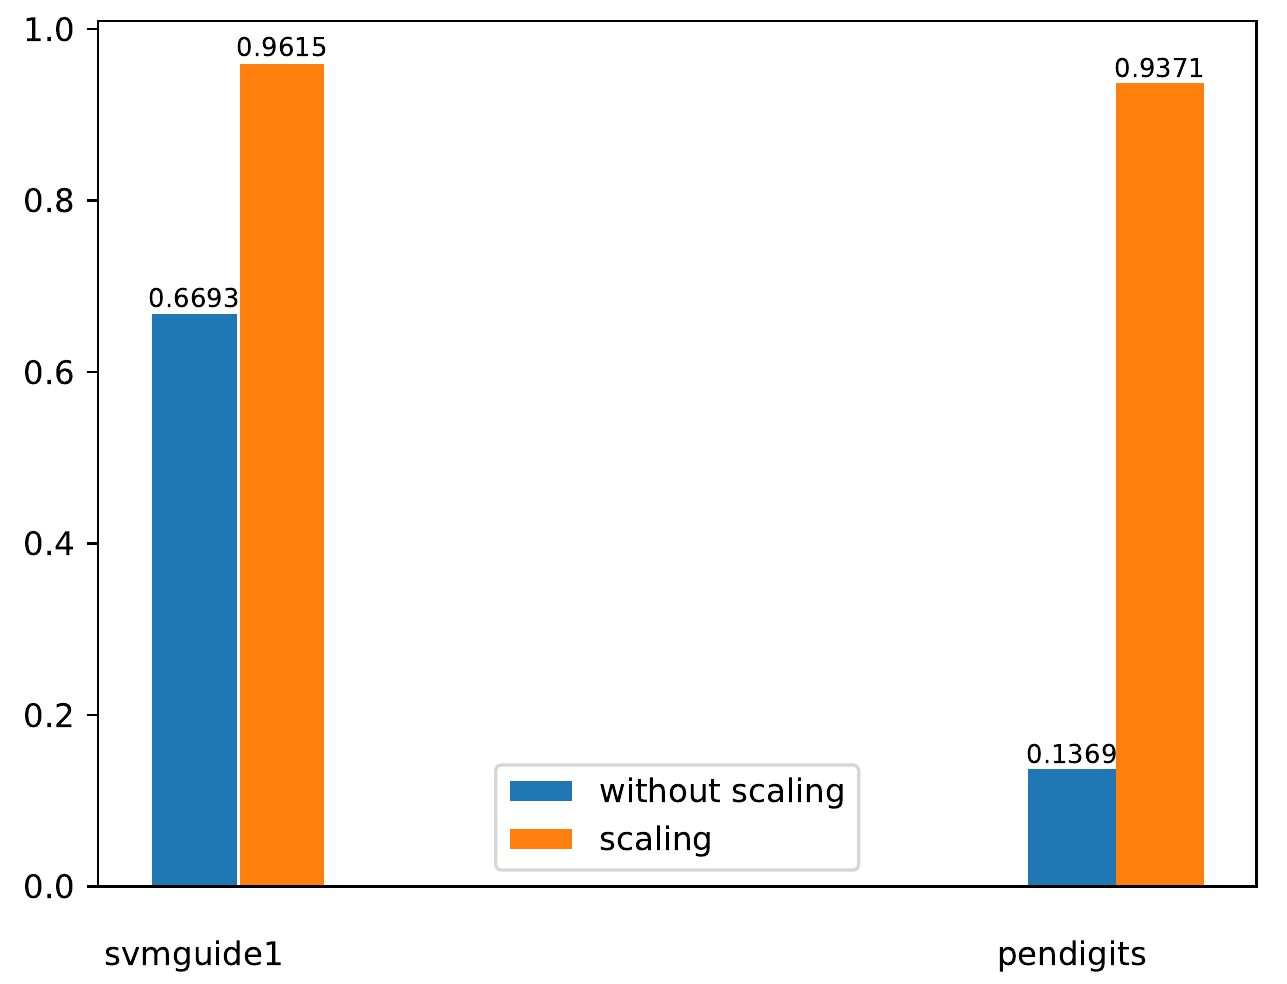
\includegraphics[width=10cm]{fig/scale.png}
 \caption{Results of SVM with scaling/non scaling}
 \label{scale}
 \end{figure}
 \subsubsection{Apply SVM with different kernels}
I tested the performace of SVM by using four basic kernels:
\begin{itemize}
\item linear: $K(x_i,x_j)=x_i^Tx_j$
\item polynomial: $K(x_i,x_j)=(\gamma x_i^Tx_J+r)^d, \gamma>0$
\item radial basis function(RBF): $K(x_i,x_j)=exp(-\gamma||x_i-x_j||^2),\gamma>0$
\item sigmoid: $K(x_i,x_j)=\tanh(\gamma x_i^Tx_j+r)$
\end{itemize}
Here, $\gamma$, $r$ and $d$ are kernel parameters. In general, the RBF kernel is a reasonable first chice for the following advantages:
\begin{itemize}
\item It can handle the
case when the relation between class labels and attributes is nonlinear.
\item The linear kernel is a special case of RBF kernel.
\item The number of hyperparameters for RBF kernel is less compared with  polynomial kernel.
\item  The RBF kernel has fewer numerical difficulties.
\end{itemize}
Here, I use the \textbf{grid.py} presented by \textbf{LIBSVM} to implement a 'grid-search' on $C$ and $\gamma$ on RBF kernel using cross-validation, which tries different pairs of $(C,\gamma)$ values and the one with the best cross-validation accuracy is picked. The results of applying 'grid-search' on the four dataset is shown in \textbf{Fig \ref{grid}}.
 
\begin{figure}[htbp]
  	\centering
  	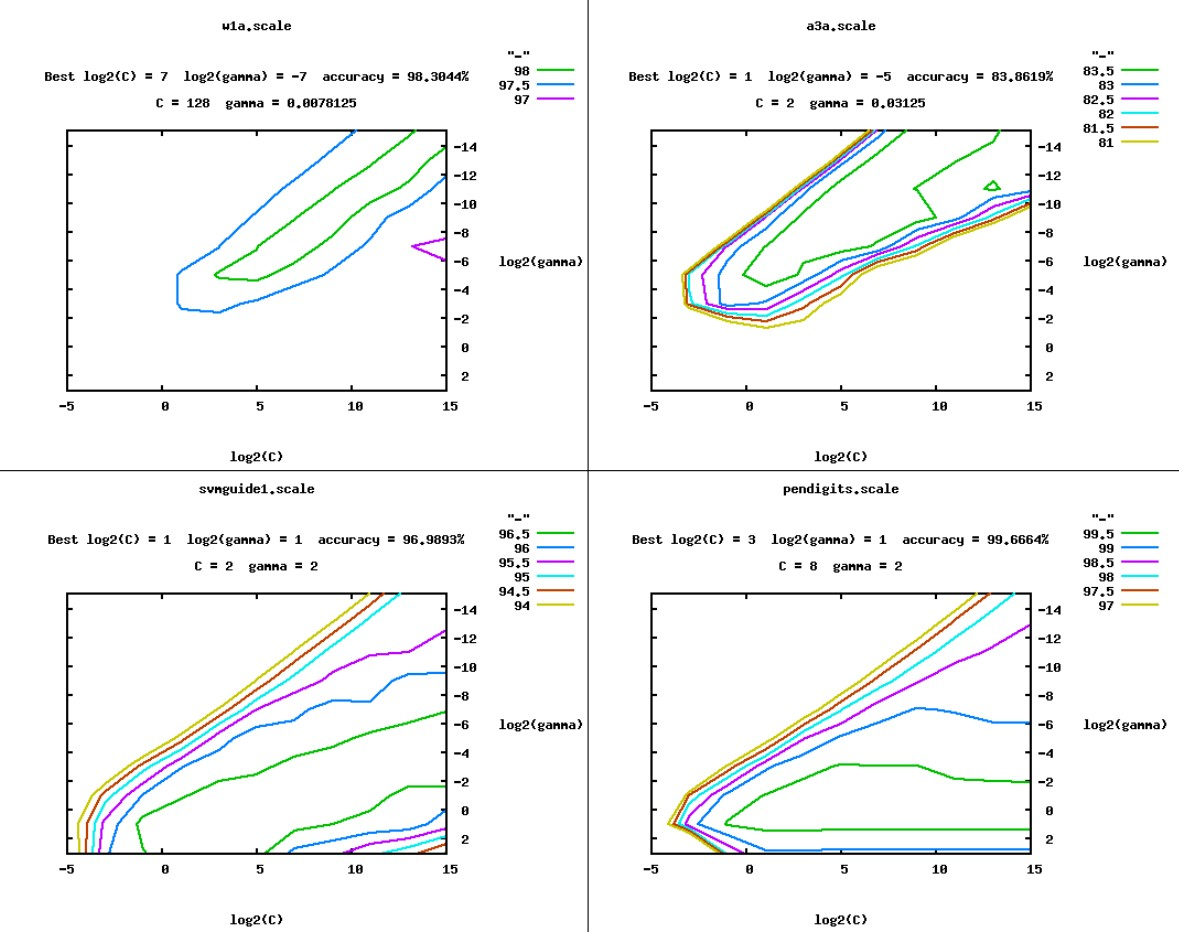
\includegraphics[width=12cm]{fig/grid.jpg}
  \caption{Applying grid search on four dataset}
  \label{grid}
  \end{figure}


 The results of applying SVM with different kernels on the four dataset is shown in \textbf{Fig \ref{kernel}}. We can see that in most cases the results obtianed by RBF kernel with grid search is the best.
 \begin{figure}[htbp]
  	\centering
  	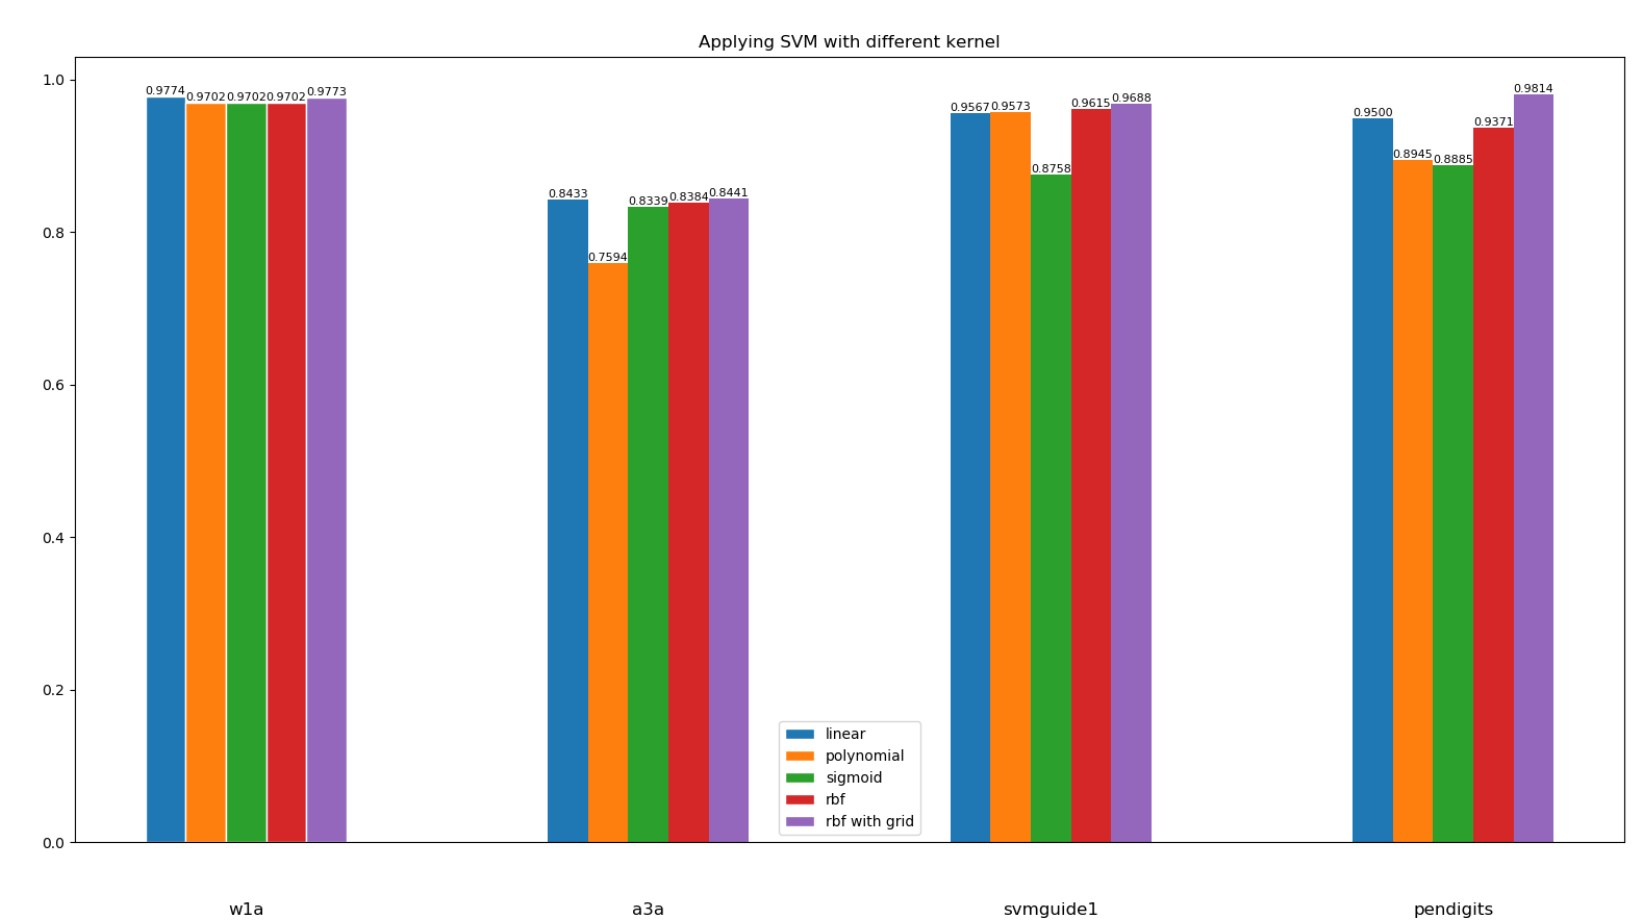
\includegraphics[width=12cm]{fig/kernel.jpg}
  \caption{Results of SVM with different kernel}
  \label{kernel}
  \end{figure}
   
\subsection{MLP results}
\subsubsection{Setting}
In this part, the code \textbf{MLP.py}, \textbf{main.py} are in the zip file, the \textbf{MLP.py} file are used to transform the file format, execute the \textbf{main.py} file, you can see the results.
\subsubsection{Apply MLP with different solvers}
The sklearn provide three solvers for weight optimization.
\begin{itemize}
\item \textbf{lbfgs} is an optimizer in the family of quasi-Newton methods.
\item \textbf{sgd} refers to stochastic gradient descent.
\item \textbf{adam} refers to a stochastic gradient-based optimizer 
\end{itemize}
The results of applying SVM with different solvers on four dataset is shown in \textbf{Fig \ref{slover}}. We can see that the \textbf{lbfgs} and \textbf{adam} performs similar, while \textbf{sgd}'s performance can vary greatly depends on the dataset.
\begin{figure}[htbp]
  	\centering
  	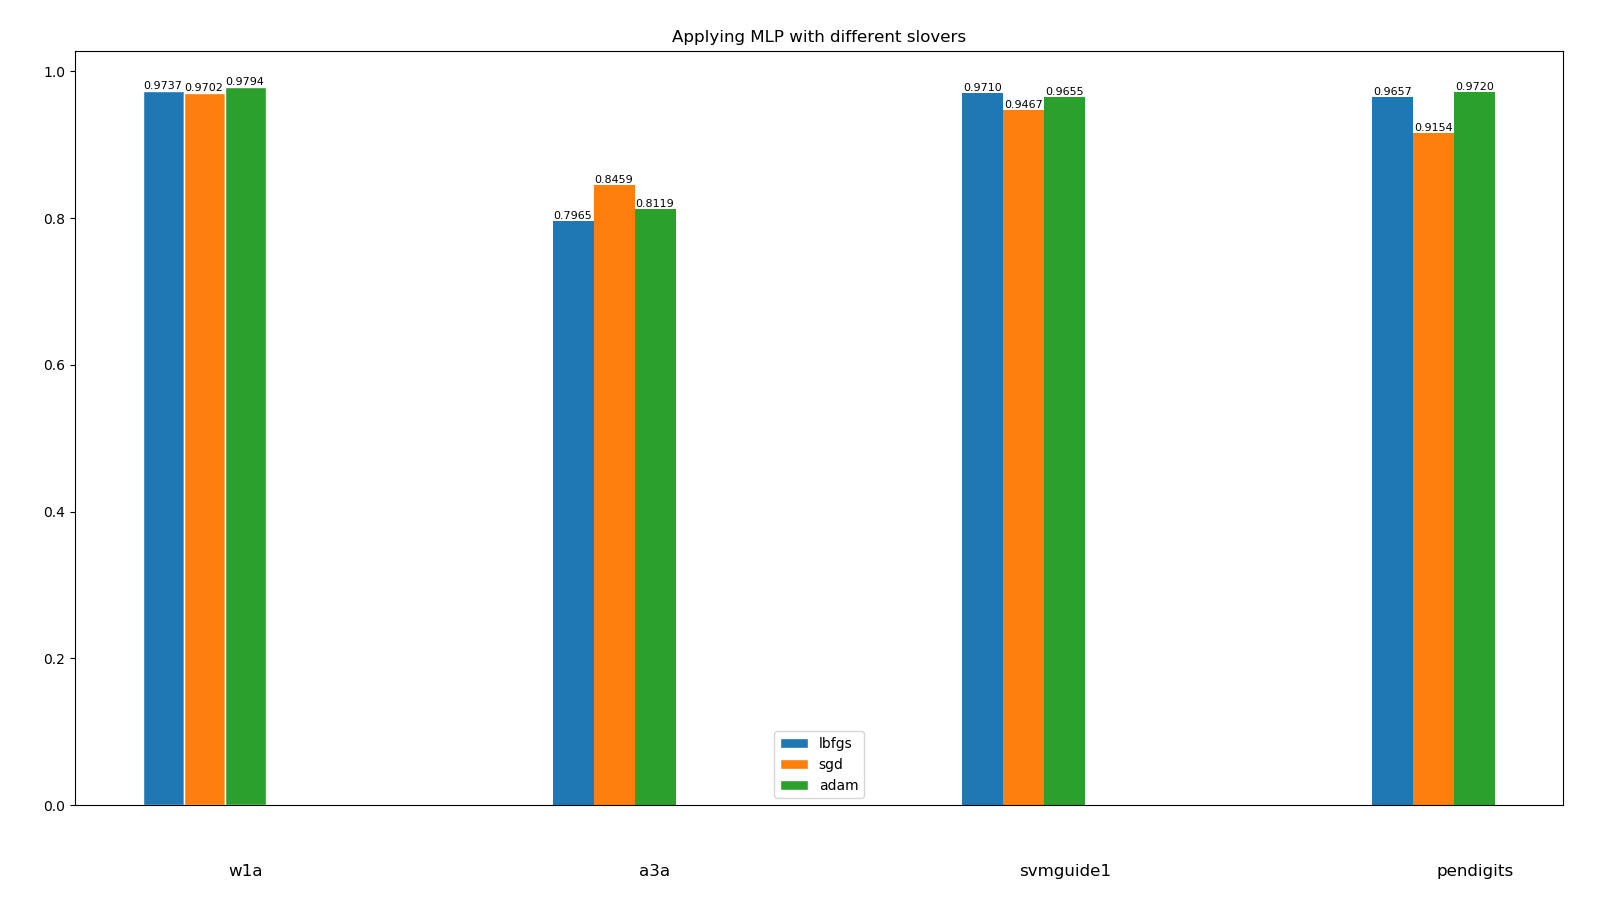
\includegraphics[width=12cm]{fig/slover.png}
  \caption{Applying MLP with different solvers}
  \label{slover}
  \end{figure}
\subsubsection{Apply MLP with different sample size}
Here I use four different sample size (0.2,0.5,0.8,1) of the training set to test the result of MLP algorithm. The result is shown in \textbf{Fig \ref{size}}.
\begin{figure}[htbp]
  	\centering
  	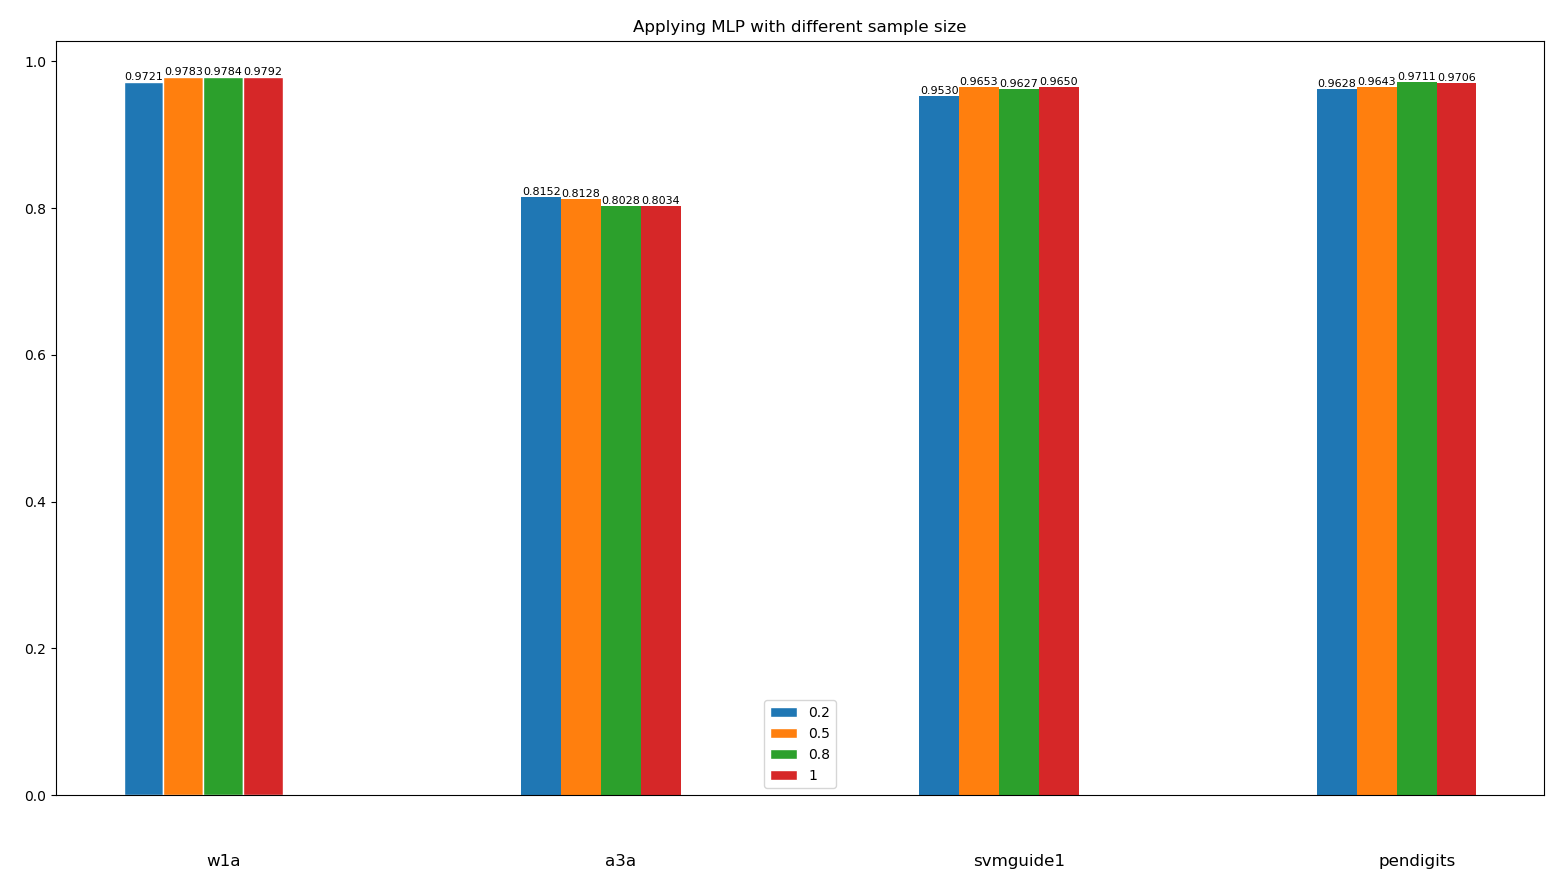
\includegraphics[width=12cm]{fig/size.png}
  \caption{Apply MLP with different sample size}
  \label{size}
  \end{figure}
\subsubsection{Apply MLP with different hidden layer sizes}
Here I use four different hidden layer size ((200,100),(100,80),(50,40),(5,2)) to test the result of MLP algorithm. The result is shown in\textbf{Fig \ref{hidden}}.
\begin{figure}[htbp]
  	\centering
  	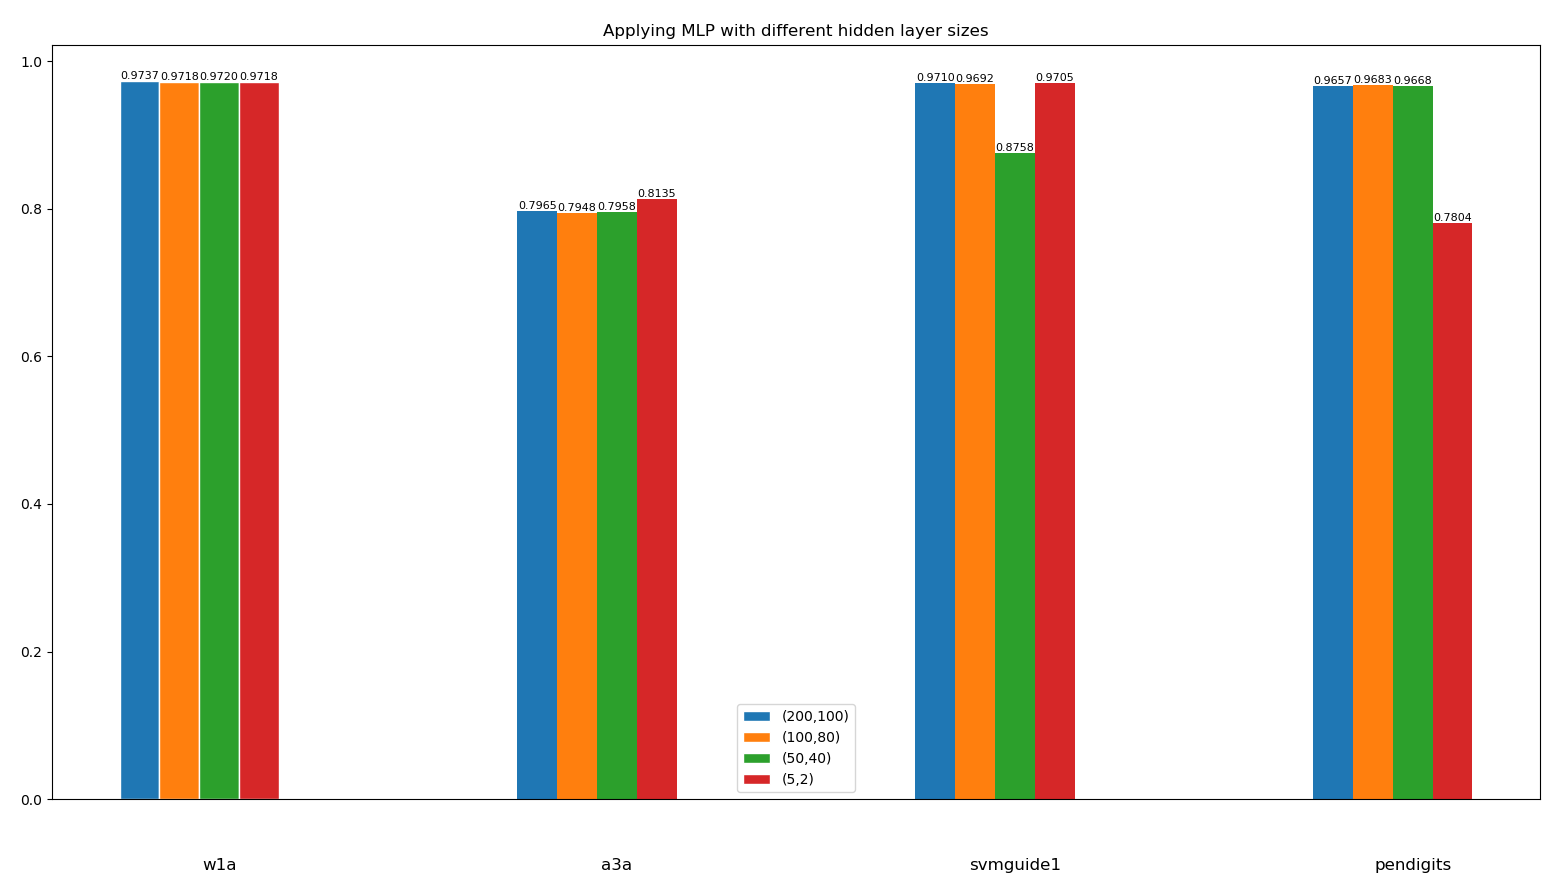
\includegraphics[width=10cm]{fig/hidden.png}
  \caption{Applying MLP with different hidden layer sizes}
  \label{hidden}
  \end{figure}

\subsection{Comparsion}
By comparing the best result obtained by SVM and MLP, we can see that for small scale dataset, their performace are similar. As is shown in \textbf{Fig \ref{compare}}.
\begin{figure}[htbp]
    	\centering
    	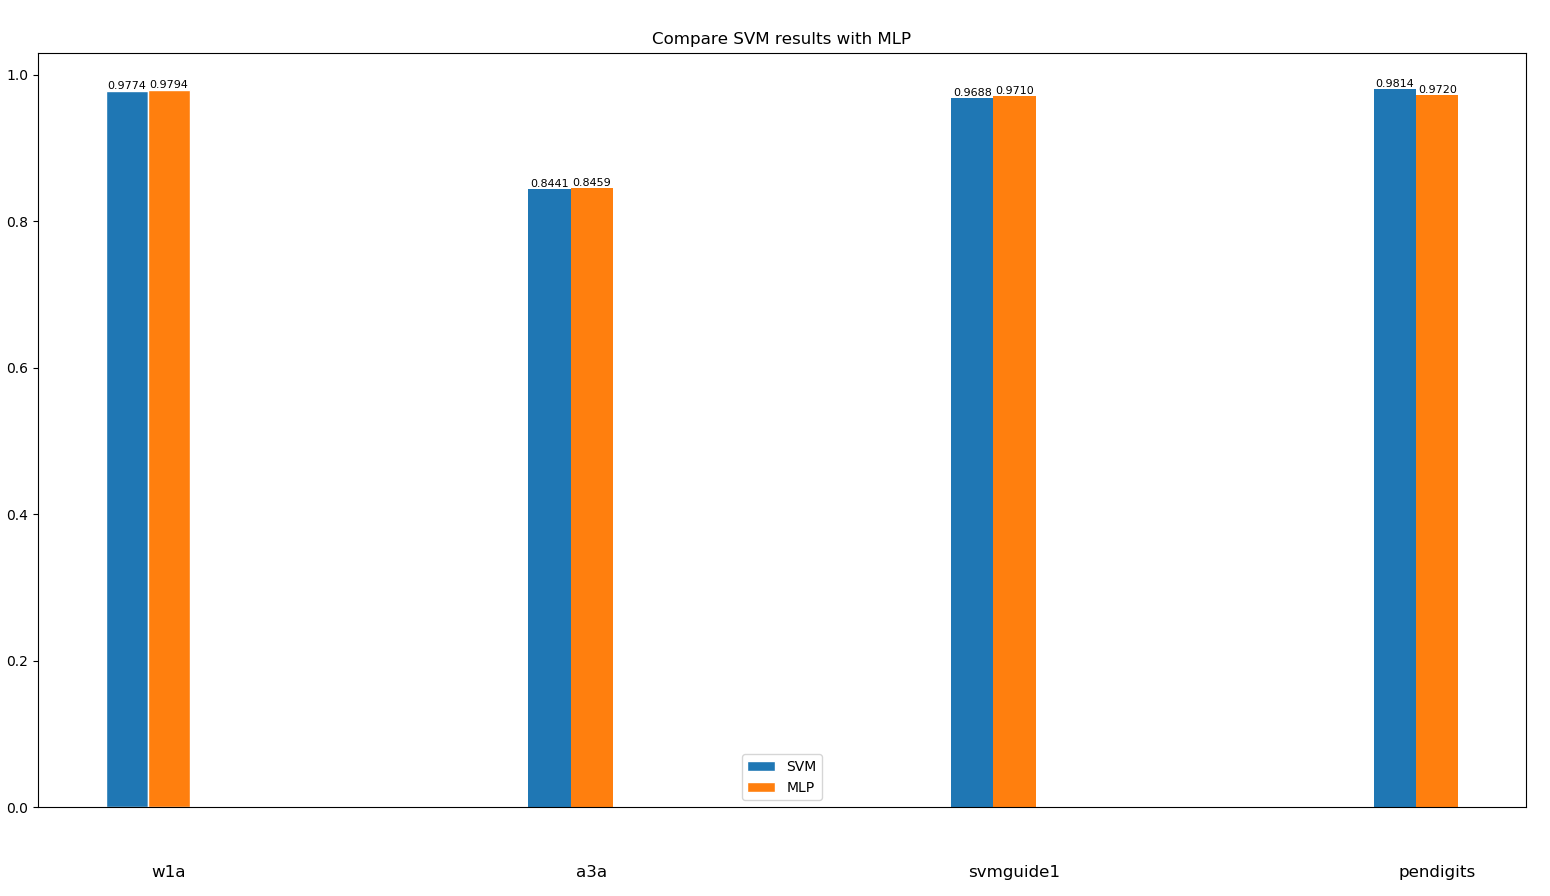
\includegraphics[width=12cm]{fig/compare.png}
    \caption{Compare SVM results with MLP}
    \label{compare}
    \end{figure}
\section{Bonus}
\subsection{Settings}
Here the code \textbf{SVM.py} is in the zip file, I didn't include the dataset since it's too large. Putting the CIFAR10 dataset in the right path, execute the \textbf{SVM.py} file, you can see the results.
\subsection{Results}
Here, I select \textbf{CIFAR10} dataset, which consists of 32*32 natural image dataset with 10 categories. \textbf{Fig \ref{CIFAR}} are the classes in the dataset, as well as 10 random images from each. Overall there are 50000 images with 5000 images for each class. 
\begin{figure}[htbp]
  	\centering
  	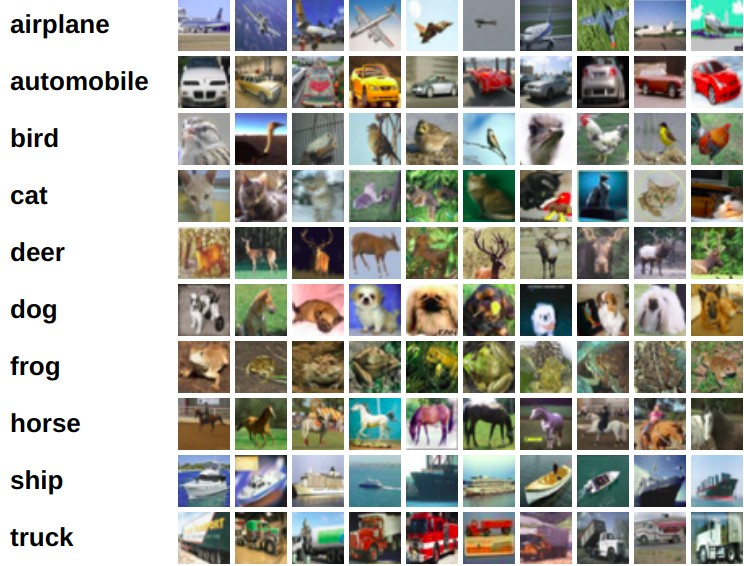
\includegraphics[width=12cm]{fig/CIFAR.jpg}
  \caption{Overview of the CIFAR10 dataset}
  \label{CIFAR}
  \end{figure}
I applied SVM with RBF kernel on this dataset and the results are shown in \textbf{Table \ref{bonus}}. We can see that the results is very poor, the overall accuracy is 9.73 \%.  It seems that the SVM just randomly pick a category for each testing image. While according to the dataset website, they are 18\% test error without data augmentation by using convolutional neural network.

  
  
 \begin{table}[htbp]
 \centering
 \caption{Results of applying SVM on CIFAR10}
 \label{bonus}
 \begin{tabular}{lclclcl}
 \hline
  features& details &	accuracy	   \\ \hline
  category 0 & 13 of 984 test values correct. & 0.0132113821138\\

  category 1 & 34 of 1007 test values correct. & 0.0337636544191\\

  category 2  & 8 of 1010 test values correct & 0.00792079207921\\

  category 3 & 14 of 995 test values correct. & 0.0140703517588\\

  category 4 & 1 of 1010 test values correct. & 0.000990099009901\\

  category 5 & 16 of 988 test values correct.  & 0.0161943319838\\

  category 6 & 701 of 1008 test values correct. & 0.695436507937\\

  category 7 & 18 of 1026 test values correct. & 0.0175438596491\\

  category 8 & 14 of 987 test values correct.& 0.0141843971631\\

  category 9 & 154 of 985 test values correct. & 0.156345177665\\
overall & 973 of 10000 test values correct. &  0.0973
  
 \end{tabular}
 \end{table}
 
 \subsection{Strengths and weaknesses of SVM on big data sets}
 \subsubsection{Weaknesses}
 \begin{itemize}
 \item Most of the kernel matrix $K$ is a $n*n$ matrix where n is the number of the data, which means storing the kernel matrix requires memory that scales quadratically with the size of the data. Also, the training time for traditional SVM algorithms also scales superlinearly with the number of data points. So these SVM algorithms aren't feasible since they require too much memories and are kind of slow.

\item Before applying SVM to a real problem, you have to choose the right kernel, which means you have to provide the true structure of the data as an input, while other algorithms, like neural networks or random-forests, try to automatically find the structure. Also, finding the structure of big data set is difficult in many cases. Of course people can use some well-difined kernels but tune the parameters for these kernels and the C parameter can be time consuming.
 \end{itemize}
  \subsubsection{Strengths}
  \begin{itemize}
  \item We can perform kernel approximation uses the Nystrom approximation (Williams and Seeger 2001). This is a way to approximate the eigenvalues/eigenvectors of a large matrix using a smaller submatrix. So that the size of kernel matrix can be greatly reduced. 
  \item We can approximate the optimization problem with a set of smaller subproblems. For example, using stochastic gradient descent on the primal problem. So that the training time can be greatly reduced.
  \item There are many SVM applications which can handle big data sets like \textbf{LaSVM} which uses online approximation to approximate SVM solver. As is shown in \textbf{Fig \ref{Lasvm}}, LASVM requires considerably less memory than a regular SVM solver. This becomes a considerable speed advantage for large training sets. 
  \begin{figure}[htbp]
    	\centering
    	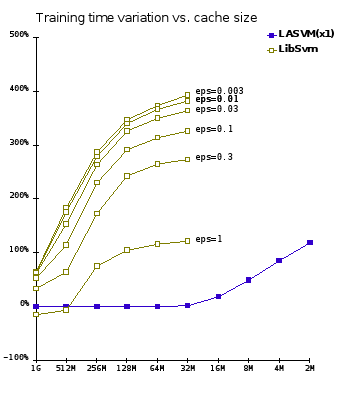
\includegraphics[width=12cm]{fig/lasvm.png}
    \caption{Compare LaSVM with LibSVM}
    \label{Lasvm}
    \end{figure}
  \end{itemize}
  
  
  \section{Reference}
  LIBSVM. Chih-Chung Chang and Chih-Jen Lin (https://www.csie.ntu.edu.tw/~cjlin/libsvm/)\\
  Williams and Seeger (2001). Using the Nystroem method to speed up kernel machines.\\
  CIFAR10: (http://www.cs.utoronto.ca/~kriz/cifar.html)\\
  LaSVM. leon.bottou.org (http://leon.bottou.org/projects/lasvm)
 
\end{document}






